\documentclass[tikz]{standalone}

\begin{document}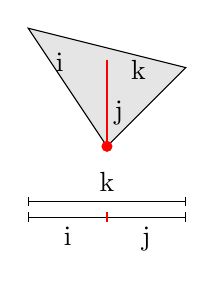
\begin{tikzpicture}
\filldraw[fill=gray!20,draw=black]
 (0,0) -- node[above=-2,pos=.4] {i} (1,-1.5)
       -- node[above,pos=.15] {j} (2,-.5)
       -- node[below=-2,pos=.3] {k} (0,0) -- cycle;

% separatrix
\fill[red] (1,-1.5) circle (2pt);
\draw[thick,red] (1,-1.5) -- (1,-.4);

\begin{scope}[yshift=-2.3cm]
\draw (0,.1) -- node[above] {k} (2,.1);
\draw (0,-.1) -- node[below] {i} (1,-.1) -- node[below] {j} (2,-.1);
\foreach \x in {0,2}
  \draw[black] +(\x,.04) -- +(\x,.16);
\foreach \x in {0,2}
  \draw[black] +(\x,-.04) -- +(\x,-.16);
\draw[red,thick] +(1,-.04) -- +(1,-.16);
\end{scope}
\end{tikzpicture}\end{document}
